% flashcards-title: Double number line for a bead bracelet with one missing value
% flashcards-desc: Two horizontal number lines with their zeros aligned. The top line, labeled silver, is marked 0, 2, 4, 6, 8. The bottom line, labeled wooden, is marked 0, 5, 10, question mark, 20. Dashed vertical guides link each aligned pair of marks; the question mark sits directly below the 6 on the silver line.
\documentclass[tikz]{standalone}
\usetikzlibrary{arrows.meta,patterns}

\definecolor{qraNavy}{HTML}{17324D}
\definecolor{qraBlue}{HTML}{2B6CB0}
\definecolor{qraGold}{HTML}{B7791F}
\definecolor{qraPale}{HTML}{EAF2F8}
\definecolor{qraGray}{HTML}{5C6773}

\tikzset{
  qra axis/.style={draw=qraNavy, line width=1.2pt},
  qra tick/.style={draw=qraNavy, line width=1pt},
  qra guide/.style={draw=qraGray, densely dashed, line width=0.8pt},
  qra counter/.style={circle, draw=qraNavy, fill=qraPale, line width=0.9pt, minimum size=7mm, inner sep=0pt},
  qra label/.style={font=\sffamily\bfseries, text=qraNavy},
  qra small label/.style={font=\sffamily, text=qraNavy},
}

\begin{document}
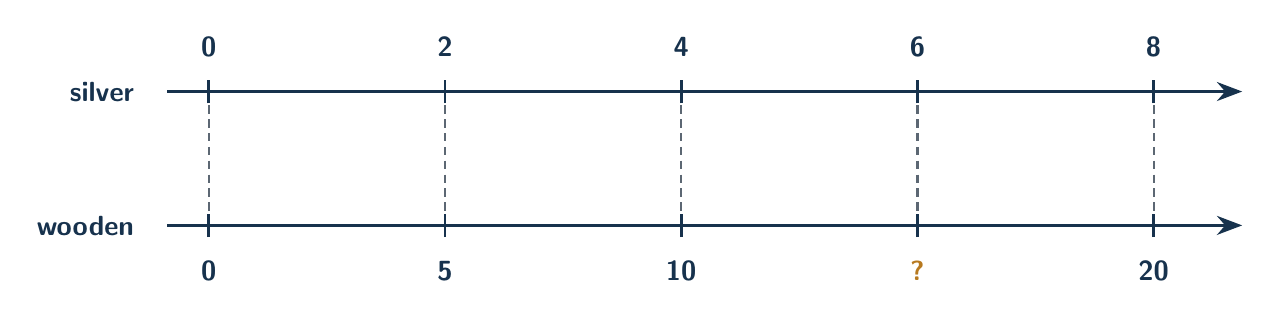
\begin{tikzpicture}[x=1.5cm]
  % Dashed pairing guides first, so lines and ticks paint over them
  \foreach \i in {0,...,4} \draw[qra guide] (\i*2,1.7) -- (\i*2,0);
  % Top line: silver
  \draw[qra axis, -{Stealth[length=3.2mm]}] (-0.35,1.7) -- (8.75,1.7);
  \foreach \i in {0,...,4} \draw[qra tick] (\i*2,1.55) -- (\i*2,1.85);
  \foreach \i/\v in {0/0,1/2,2/4,3/6,4/8}
    \node[qra label, above=5pt] at (\i*2,1.85) {\v};
  \node[qra label, anchor=east] at (-0.55,1.7) {silver};
  % Bottom line: wooden, with the missing value highlighted
  \draw[qra axis, -{Stealth[length=3.2mm]}] (-0.35,0) -- (8.75,0);
  \foreach \i in {0,...,4} \draw[qra tick] (\i*2,-0.15) -- (\i*2,0.15);
  \foreach \i/\v in {0/0,1/5,2/10,4/20}
    \node[qra label, below=5pt] at (\i*2,-0.15) {\v};
  \node[qra label, text=qraGold, below=5pt] at (6,-0.15) {?};
  \node[qra label, anchor=east] at (-0.55,0) {wooden};
\end{tikzpicture}
\end{document}
